\section{Франкенвордические неформологизмы}

Ужачно = удачно + ужасно --- ужасно удачно\\

\emph{Аналогично:} уржачно\\

Бабаня --- \emph{ну тут всё ясно, а вот следующее --- это ещё одно слово с 2-мя буквами ё:} Тётёля

\begin{figure}[ht!]
    \centering
    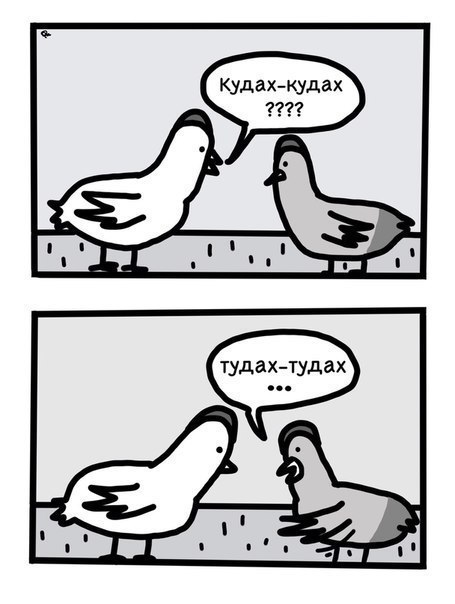
\includegraphics[width=0.6\textwidth]{tudakh}
    \caption{Alice, stop using drugs!}
\end{figure}

Идея: написать маленький рассказ из набора фраз на одну букву.\\
Главное условие: не меньше 3-х слов подряд должны быть на одну букву.

\subsection{Как заставить всех людей строить странные предложения и не стать психом}
\emph{Собственно весь "рассказ" --- это просто диалог двух обычных квазисреднестатистических людей, что является реализацией ещё одной идеи по попутному написанию литературных творений в любой наперёд заданной форме.}

\begin{flushleft}\parskip1em
    \emph{Я прочувствовал дух однобуквенного высказывания:}
    Василий Васильевич Васильев всё время валял вал\\
    --- Всё валяешь вал?\\
    --- Валяю вал\\
    --- Вандал! Варварство! Ватман!\\
    --- Ватман?\\
    --- Вероломство!\\
    Вдохновленный вандал всё валял, валял... Великолепно валял вал.

    --- Вы вдохновенно ввалились в...\\
    --- ...высказывание?\\
    --- Возможно.\\
    --- Вероятно вы верно вещаете.\\
    --- Ворчанием воздержитесь воздавать возведённое великолепие.

    \emph{"Великолепное ворчание всё время воздаёт величественную возню!"}
    \vspace*{-1em}\begin{flushright}
        Великий Воитель
    \end{flushright}

    \emph{Вычурно вы выводите все ваши высказывания, владыка!}

    \emph{Владею, верую, воздаю!}

    \emph{Вмиг вмешиваете вменяемость в виртуально вывитую вещь.}

    \emph{Виртуозно и вычурно вывернул!}

    \emph{Наитивно навыком научились науськивать наши недра неких надумок.}

    \emph{Адски азартно аплодирую!}

    \emph{Да, довольно дельно думать научился на наших беседах без больших затрат за звено времени возымевшимся в своём распоряжении.}

    \emph{Дык, договорились делать данный диалог в выбранной высказывательной форме.}

    \emph{Хорошо хоть хочу делать данный диалог.}

    \emph{Этот эдакий энтузиазм иссякнуть или исчезнуть вполне внезапно возымеет --- надо наибольшее напряжение проявить при проектировании фантазируемых фурорных фраз.}

    \emph{Очень Ожегова освежить снова следует сейчас. Коль когда костноязычно говоришь --- голова гудит}

    По простецкой по причине\\
    Коль когда костноязычишь\\
    Говоришь гундёж гремучий\\
    Ты теперь тут получай

    \vskip1em

    \emph{[полубелый стих]}\\
    Трудно трутню трюизмами\\
    Изысканные измышления изваять.\\
    Посему повелеваем вам\\
    Книжки купленны читать

    Загнуть заросли загубленных\\
    Мыслей мешает мука моя:\\
    Придумки повес пришлашённых\\
    Расхоже расценила моя семья

    Туманно тучи толпятся в ночи\\
    Ты тоже теперь его не ищи\\
    Закинул зелёную зарисовку подальше\\
    Не будет не будет теперь всё иначе\\

    \vskip1em

    \emph{\anttf{на этом месте мы раскрыли причину того, почему в песнях такая муть встречается. 
    Мы раскрыли их зловещий план! --- Теперь мы гребём бабло! и выбрали девиз для мёртвой сосны}}

    \emph{\anttf{Тут просто открыл словарь и читаю слова на одной стр:}}\\
    \emph{Дубильщик дубасит дрянной дубиной дрябоый дуализм дублируя дублоны дружинника...}

    \emph{Пошёл поток прекрасных новых неформальных неологизмов!}

    \emph{"Фокусник Фёдор фелонит"}

    \emph{феерично фыркнул фуникулёрщик}
\end{flushleft}
% немного рекламы
\begin{figure}[ht!]
    \centering
    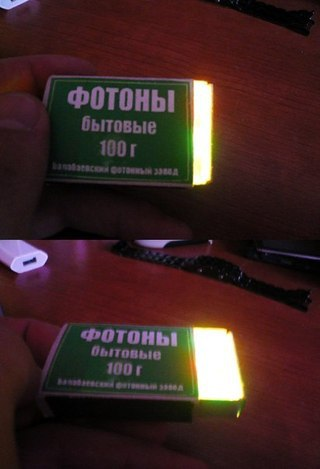
\includegraphics[width=\textwidth]{fot}
    \caption{Свежие фотоны у вас меньше чем за 8 минут!}
\end{figure}

\vskip4em

\framebox[0.9\textwidth][c]{
    Здесь могла быть ваша реклама, но нет!
}
